\chapter{Généralités sur l'optimisation et sur les méta-heuristiques}

\section*{Introduction}

L'Intelligence Artificielle (IA) est un ensemble de techniques
informatiques qui permettent à l'ordinateur de résoudre des problèmes
complexes nécessitant un raisonnement intelligent comme celui de
l'être humain, ou même l'aptitude à acquérir, à apprendre et à utiliser des
connaissances. Le terme IA a été introduit la première fois en 1956 lors
d'une conférence sur l'intelligence des ordinateurs.

Parmi les domaines les plus importants de l'intelligence artificielle, on
trouve la fouille de données (Data Mining), la technologie des agents, la
recherche d'information...etc, qui nécessitent des méthodes spécifiques pour résoudre des problèmes d'optimisation complexes.

\section{Problème d'optimisation}
C'est la recherche, parmi un ensemble de solutions, de celle qui maximise ou minimise une fonction objectif mesurant la qualité de cette solution. Cela revient à chercher un optimum global. Un tel problème fait appel à une ou plusieurs techniques d'optimisation.

\section{L'optimisation}
C'est une discipline de la recherche opérationnelle qui a vu le jour au $20^{ème}$ siècle et qui consiste à choisir, parmi plusieurs possibilités, celle qui répond le mieux à un ou plusieurs critères souhaités.\\

L'outil mathématique intervient dans la résolution des problèmes d'optimisation en les définissant d'une manière formelle et adéquate. 

Il existe deux types d'optimisation, l'optimisation combinatoire qui traite les problèmes à variables discrètes, et l'optimisation continue qui traite les problèmes à variables continues. 

On distingue dans chacune de ces optimisations deux sous classes:
\begin{itemize}
	\item l'optimisation mono-objectif qui cherche à optimiser un seul critère,
	\item l'optimisation multi-objectif qui cherche à optimiser plusieurs critères souvent contradictoires. Par exemple, visiter le plus grand nombre de villes au moindre coût possible. Ce conflit nous pousse à imposer un ordre de préférence entre les critères en définissant une relation d'ordre partiel appelée relation de dominance. 
\end{itemize}

De plus, il existe des problèmes d'optimisation avec et sans contraintes. Une contrainte cherche à restreindre l'espace de recherche et à vérifier l'admissibilité d'une solution sauf qu'elle ne mesure pas la qualité de la solution. 



%\parbox[c][0em][s]{\textwidth}{}

%\vspace{-1em}

\subsection{L'optimisation combinatoire}
Elle consiste à trouver, dans un ensemble discret, une solution parmi les meilleures réalisables. En général, cet ensemble de solutions est fini mais comporte un très grand nombre d'éléments, et il est décrit de manière implicite, c'est-à-dire par une liste  relativement courte de contraintes que doivent satisfaire les solutions réalisables. La notion de meilleure solution est définie par une fonction objectif à maximiser ou à minimiser.

\vspace{1em}

Nous nous intéressons dans ce travail à l'optimisation continue.
\subsection{L'optimisation continue}

Appelée aussi optimisation globale, consiste à trouver les meilleures solutions possibles $x^* \in X$ selon un ensemble de critères
$F = \{f_1,...,f_n\}$. Les critères, appelés fonctions objectifs, sont exprimés sous
forme de fonctions mathématiques. Une fonction objectif est une fonction mathématique
telle que :
$$f : D \subset \mathbb{R}^n \mapsto \mathbb{R},$$ 


où $D$ est l'ensemble des points admissibles de l'espace de recherche.

L'optimisation continue fait appel à la notion de continuité d'une fonction mathématique que nous devons expliquer avant de rentrer dans les détails.

\subsubsection{$\bullet\quad$Continuité d'une fonction en un point\cite{continue}}
Soit $\alpha$ un réel de $D$.

\begin{itemize}
	\item f est continue en $\alpha$ si et seulement si $\lim\limits_{x \rightarrow \alpha}f(x)=f(\alpha)$
	\item f est continue en $\alpha$ si et seulement si $\lim\limits_{h \rightarrow 0}f(a + h)=f(\alpha)$
\end{itemize}


\subsubsection{$\bullet\quad$Continuité d'une fonction sur un intervalle\cite{continue}}

\begin{itemize}
	\item $f$ est continue sur $D$ si et seulement si $f$ est continue en chaque réel $\alpha$ de $D$.
\end{itemize}


\vspace{1em}

Dans le cas de l'optimisation d'un seul critère $f$, un optimum peut être
le maximum ou le minimum de la fonction \cite{Momin_Yang_2013}.

Les problèmes d'optimisation
globale (continue) sont la plupart du temps définis comme des problèmes de
minimisation, car maximiser $f$ revient à minimiser $-f$ \cite{cvijovic1995taboo}.

\vspace{1em}

La vraie solution optimale pour un problème d'optimisation peut être
un ensemble $x^* \in D$  de tous les points optimaux de $D$,
comme elle peut être aussi une seule valeur minimale ou maximale, et cela parce qu'on peut avoir plusieurs ou même une infinité de solutions optimales, cela dépend du
domaine qui nous intéresse de l'espace de recherche.

\vspace{1em}

La tâche de n'importe quel bon algorithme d'optimisation globale
est de trouver l'optimum global ou au moins des solutions sous-optimales (optimums locaux), c'est-à-dire des optimums globaux pour un sous-domaine du domaine de définition de la fonction\cite{Momin_Yang_2013}.

\vspace{1em}

La différence entre un optimum global et un optimum local apparait dans la figure suivante.

\begin{figure}[H]
	\centering
	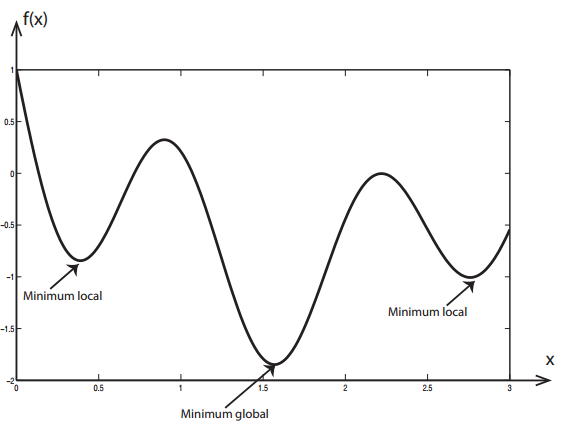
\includegraphics[width=0.6\textwidth,keepaspectratio]{diff_optGlobal_optLocal}
	\caption[Différence entre un optimum global et un optimum local]{Différence entre un optimum global et un optimum local \cite{boussaid}}
\end{figure}

Les fonctions objectifs peuvent être continues, discontinues,
linéaires, non-linéaires, convexes, non-convexes, uni-modales,
multi-modales, séparables ou non-séparables\cite{Momin_Yang_2013}.

\begin{itemize}
	\item La séparabilité mesure la difficulté d'une fonction. En général, une fonction séparable est plus ou moins facile à minimiser en la comparant avec une autre non-séparable car chaque variable d'une fonction séparable est indépendante des autres. Du coup, la fonction peut être écrite sous forme d'une somme de plusieurs fonctions, chacune à une seule variable\cite{Momin_Yang_2013}.
	\item Le nombre de pics dans le graphe d'une fonction correspond à sa modalité. Une fonction multi-modale est une fonction qui admet plusieurs optimums locaux. Ce type de fonctions est difficile à minimiser car l'algorithme peut stagner dans un optimum local et ne plus en sortir. 
	\item La difficulté d'un problème augmente avec l'augmentation de sa dimension, ce qui représente une barrière pour la plupart des algorithmes d'optimisation. 
\end{itemize}

Les classes des problèmes d'optimisation continue sont variées, d'où la difficulté de trouver une méthode de résolution générale efficiente. C'est la raison pour laquelle nous nous intéressons dans ce travail aux problèmes d'optimisation continue mono-objectif, sans contraintes et de minimisation.

A l'augmentation de la taille du problème, ce dernier devient plus difficile à résoudre et ne peut pas être résolu de manière exacte dans un temps raisonnable, d'où l'intérêt des méthodes approchées qui évitent l'explosion combinatoire par l'exploration partielle de l'espace de recherche mais d'une manière intelligente.\\

\section{Les méta-heuristiques}

Ce sont des algorithmes génériques qui utilisent des
heuristiques pour donner des solutions approchées à des problèmes
complexes en utilisant une approche guidée par une technique
spécifique.

Les méta-heuristiques se présentent sous deux catégories, celles qui
ne sont pas bio-inspirées telles que la recherche Tabou et la recherche
dispersée, et celles qui le sont telles que l’algorithme génétique et les
algorithmes issus de l’intelligence en essaim (par exemple les algorithmes des
colonies de fourmis et d'essaims d’abeilles qui ont été initialement
conçus pour des problèmes combinatoires et aussi les algorithmes Bat Algorithm (BA) et Particle Swarm Optimization (PSO) qui ont été développés pour des problèmes continus).

Toutes les méta-heuristiques comportent deux stratégies de
recherche :

\begin{itemize}
	\item l'intensification par recherche locale dans une seule région de l'espace de recherche,
	\item la diversification qui consiste à changer de région pour en explorer d'autres.
\end{itemize}

L'importance de la stratégie de recherche varie d'une méta-heuristique à une autre, cela dépend généralement des besoins souhaités:

\begin{itemize}
	\item plus d'intensification mène à une solution de meilleure qualité,
	\item plus de diversification mène à trouver une solution en un temps plus réduit,
	\item un compromis entre les deux mène à une meilleure solution en un temps plus réduit.
\end{itemize}

\section{L'intelligence en essaim}

C'est une technologie très importante de l'intelligence artificielle qui recouvre un ensemble d'algorithmes à base de population d'agents simples. Un algorithme issu de l'intelligence en essaim se base sur deux principes:

\begin{itemize}
	\item l'observation à partir des phénomènes naturels intelligents et plus précisément des comportements en groupe,
	\item la simulation des comportements collectifs des insectes (fourmis
	et abeilles) et des animaux (poissons et oiseaux) qui traduisent une intelligence collective.
\end{itemize}

Un essaim peut être vu comme étant un groupe d'agents où chacun
fait une tâche élémentaire. L'efficacité de l'essaim peut être remarquée
d'un point de vue global qui est établi grâce à l'interaction sociale entre les
agents. Cette interaction influence les comportements individuels
des agents et les pousse à apporter leur contribution pour atteindre ensemble un but global qui représente le but de l'essaim.

L'intelligence en essaim a été appliquée à plusieurs domaines:

\begin{itemize}
	\item l'optimisation combinatoire (voyageur de commerce,
	ordonnancement et planification, transport moderne,
	télécommunications, etc...),
	\item l'optimisation continue (optimisation des fonctions numériques),
	\item les applications de l'intelligence artificielle (traitement automatique
	du langage, traitement d'image et robotique),
	\item les applications de divertissement (films et jeux vidéo),
	\item la fouille de données (Data Mining),
	\item le routage dans les réseaux,
	\item les applications Web (recherche, filtrage et sécurité).
\end{itemize}

\section*{Conclusion}

Après avoir introduit le domaine de l'intelligence artificielle et plus particulièrement celui de l'optimisation, nous avons abordé la différence entre l'optimisation combinatoire et celle continue. Puis, nous avons présenté la philosophie des méta-heuristiques et de l'intelligence en essaim ainsi que ses différentes adaptations. Le chapitre suivant est consacré aux travaux réalisés par les chercheurs dans le domaine de l'optimisation continue.
